\documentclass[11pt]{article}
\usepackage[utf8]{inputenc}
\usepackage[T1]{fontenc}
\usepackage{lmodern}
\usepackage[english]{babel}
\usepackage{geometry}
\geometry{a4paper, margin=2.3cm}
\usepackage{graphicx}
\usepackage{csquotes}
\usepackage{amsmath, amssymb}
\usepackage{booktabs}
\usepackage{tabularx}
\usepackage{caption}
\usepackage{float}
\usepackage[round]{natbib}
\usepackage{titling}
\usepackage{xcolor}
\usepackage[colorlinks=true, linkcolor=blue!50!black, citecolor=blue!50!black, urlcolor=blue!50!black]{hyperref}
\graphicspath{{img/}{../figures/}}
\captionsetup{font=small, labelfont=bf}

% ---------------------------------------------------------------------------
% Key results (filled from the executed notebooks, data up to 23 October 2026)
% ---------------------------------------------------------------------------
% generated by scripts/make_report.py from data/processed/results_0*.json; do not edit
\newcommand{\NnetPM}{74}
\newcommand{\NnetOz}{68}
\newcommand{\ValOzN}{159{,}138}
\newcommand{\ValPMwithin}{99.95}
\newcommand{\VoneGood}{1}
\newcommand{\VtwoGood}{78}
\newcommand{\FlagOz}{157}
\newcommand{\FlagPM}{174}
\newcommand{\StableRatio}{1.42}
\newcommand{\CorrBefore}{0.69}
\newcommand{\CorrAfter}{0.93}
\newcommand{\FillRtwoPM}{0.94}
\newcommand{\FillRtwoOz}{0.97}
\newcommand{\RawCov}{70}
\newcommand{\CatAcc}{83}
\newcommand{\CatAccPers}{73}
\newcommand{\ShareGoodTwelve}{83}
\newcommand{\ShareGoodTwentyFour}{72}
\newcommand{\ShareGoodEEA}{14}
\newcommand{\WhoMin}{7}
\newcommand{\WhoMax}{33}
\newcommand{\TrendPM}{0.01}
\newcommand{\TrendOz}{0.25}
\newcommand{\TrendOzPct}{0.7}
\newcommand{\TrendOzP}{$<0.001$}
\newcommand{\WorstPM}{154}
\newcommand{\WorstAQI}{229}
\newcommand{\SecondAQI}{174}
\newcommand{\FireworksPM}{5.6}
\newcommand{\CovidNOtwo}{15}
\newcommand{\CovidPM}{39}
\newcommand{\PlaceboNOmin}{$-$6}
\newcommand{\PlaceboNOmax}{3}
\newcommand{\PlaceboPMmin}{$-$17}
\newcommand{\PlaceboPMmax}{8}
\newcommand{\LiveDate}{2026-10-24}
\newcommand{\LiveAQI}{29}
\newcommand{\LiveCat}{Good}
\newcommand{\LowCostExact}{75}
\newcommand{\LowCostOne}{99}
\newcommand{\VoneRFmae}{22.5}
\newcommand{\BenzeneRtwo}{0.99998}
\newcommand{\GeoPMgp}{3.23}
\newcommand{\GeoPMgpR}{0.94}
\newcommand{\GeoOzbest}{3.83}
\newcommand{\GeoOzbestR}{0.90}
\newcommand{\PopPM}{7.1}
\newcommand{\PopRatio}{1.4}
\newcommand{\FcPMopMAE}{2.41}
\newcommand{\FcPMopSkP}{16}
\newcommand{\FcPMopSkC}{21}
\newcommand{\FcPMopCov}{81}
\newcommand{\FcPMwxMAE}{1.97}
\newcommand{\FcPMwxSkP}{31}
\newcommand{\FcPMwxSkC}{36}
\newcommand{\FcPMwxCov}{81}
\newcommand{\FcOzopMAE}{6.29}
\newcommand{\FcOzopSkP}{18}
\newcommand{\FcOzopSkC}{12}
\newcommand{\FcOzopCov}{81}
\newcommand{\FcOzwxMAE}{4.42}
\newcommand{\FcOzwxSkP}{42}
\newcommand{\FcOzwxSkC}{38}
\newcommand{\FcOzwxCov}{82}


\title{Predicting the Air Quality Index with Data Science and Machine Learning\\[0.3em]\large Version 2: quality control, multi-standard indices, probabilistic forecasting and geospatial prediction}
\author{GROLLEAU Florian\\
2A Dual Diploma \\ Sciences Po Saint-Germain-en-Laye / CY TECH Engineering School}
\date{October 2026}
\pretitle{%
  \begin{center}
  
\includegraphics[height=2.5cm]{logocergy.jpg}\par\vspace{0.5cm}
  \LARGE
}
\posttitle{\end{center}}

\begin{document}

\maketitle
\begin{abstract}
Since the massive urbanization and high-density human activities phenomena, such as industrialization and overconsumption of services and goods, the global Air Quality Index (AQI) has regressed. However, the global AQI does not reflect the very localized impact and changes on a rather small geographic area. For this reason, there is a need for more accurate metrics and qualitative analysis of the AQI over smaller regions than a worldwide analysis. Thanks to the emergence of several Data Science tools and Machine Learning models, we aim for better monitoring and prediction of local AQI.

This second version rebuilds the study on public, independently verifiable data: the US EPA AirNow network (\NnetPM{} fine-particle and \NnetOz{} ozone monitors around New York, 2014 to October 2026), NOAA weather records and the UCI low-cost sensor dataset of an Italian city. It shows that the data used in version 1 had been read on the wrong scale and contained silent sensor failures, implements and validates a multi-standard AQI engine, separates emission trends from weather, attributes pollution episodes (wildfire smoke, fireworks, the COVID-19 lockdown), forecasts the AQI with calibrated uncertainty and maps it continuously between monitors.
\end{abstract}

\newpage
\tableofcontents
\newpage

% ===========================================================================
\section{What is AQI?}
% ===========================================================================

By the acknowledgement of global climatic changes, the question of the quality of the air, and mainly its troposphere layer, emerged. As a matter of fact, the troposphere represents 90 percent of the total mass of the atmosphere and contains almost the entire volume of water vapor \citep{olschewski2025}. Moreover, according to the state of progress of the life sciences, every living being interacts within this critical layer of the atmosphere. For this reason, the quality of the air matters and, in the current position, constitutes a major challenge in the preservation of ecosystems and human societies. Among the several factors which affect air quality, human pollution is considered as the one affecting the most the values of air quality \citep{beig2010}. Indeed, ``It can pose a serious threat to human health if it exceeds the permissible limit'' (WHO, 2000; USEPA, 2008). Every year, over 2 million premature deaths are reported due to air pollution, and ``the effect of urban (outdoor/indoor) air pollution is caused by burning of solid fuels'' (WHO, 2000, 2002, 2005). As the challenges for a healthier air quality arose, the need for a more rigorous metric designed for scientific monitoring emerged: the AQI. Since the official publication by the US Environmental Protection Agency of its Pollutant Standards Index in 1976, renamed Air Quality Index in 1999, its worldwide usage has significantly increased.

\subsection{Definition and Purpose}

Supporting the WHO air quality guidelines \citep{who2021}, the AQI has been established as a standard for most countries in their aim of monitoring the air quality. Particularly, it has been assessed that ``more than half of the air pollution-driven disease burden is borne by the population of developing countries'' \citep{beig2010}. This strengthens the prospects for improving air quality, as these countries are undergoing profound technological and economic transformations. A definition of the AQI has been provided by the Florida Department of Environmental Protection, which defines the AQI as a ``tool for reporting daily air quality. It tells you how clean or polluted your air is and what associated health effects might be a concern for you. The AQI focuses on health effects you may experience within a few hours or days after breathing polluted air. It takes all the monitored pollutants and relates them to a single-scale value to indicate air quality.'' It is usually a scale of 0 to 500; the higher the AQI value, the greater the level of air pollution and the greater the health concern. However, there isn't a worldwide harmonized scale of standards; for example, Australia's environmental agency uses the NEPM (National Environment Protection Measure), which considers an AQI in the range of 67 to 99 as ``fair,'' while in Europe, an index of 75 to 100 is considered as ``high polluted air.''

Moreover, numerous countries use a unique mathematical equation to measure the AQI (such as Canada's Air Quality Health Index, Malaysia's Air Pollution Index, and Singapore's Pollutant Standards Index). Considering a more physics-oriented definition, the AQI ``requires an air pollutant concentration over a precise averaging period, obtained from an air monitor or model. Taken together, concentration and time represent the dose of the air pollutant. Health effects corresponding to a given dose are established by epidemiological research. Its air quality index values are typically grouped into ranges.''

\begin{figure}[H]
    \centering
    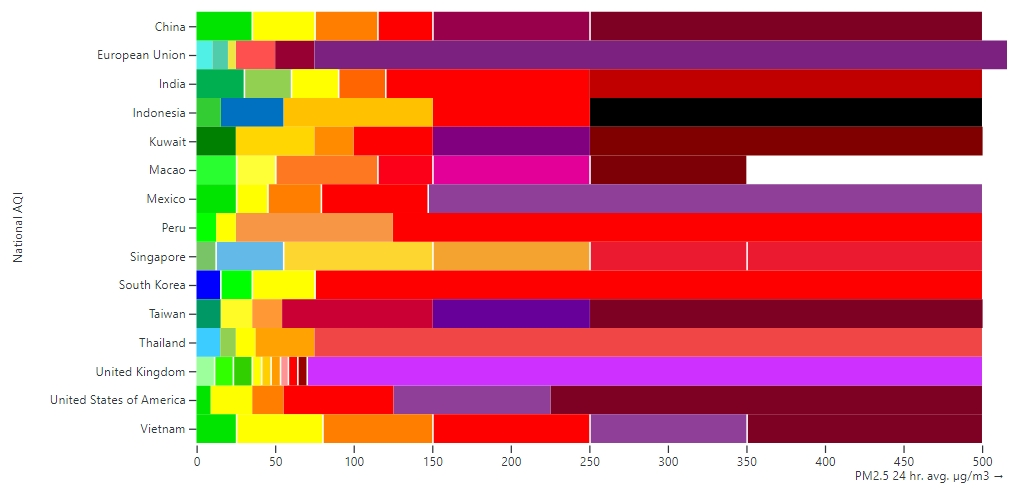
\includegraphics[width=0.95\textwidth]{airqualitystandards.jpeg}
    \caption{Summary of air quality standards for different countries (OpenAQ, 2024).}
    \label{fig:air_quality_standards}
\end{figure}

As shown in Figure~\ref{fig:air_quality_standards}, each range is assigned a descriptor, a color code, and a standardized public health advisory. The pollutants that are largely prioritized in the monitoring process are ozone (O$_3$), particulates (PM$_{2.5}$), sulfur dioxide (SO$_2$), carbon monoxide (CO), and nitrogen dioxide (NO$_2$). Since the World Health Organization has not published an index that is universally used, we use by default the American EPA scale of the AQI shown in Figure~\ref{fig:aqi_usa}, and compare it with the European and Canadian conventions in Section~\ref{sec:standards}.

\begin{figure}[H]
    \centering
    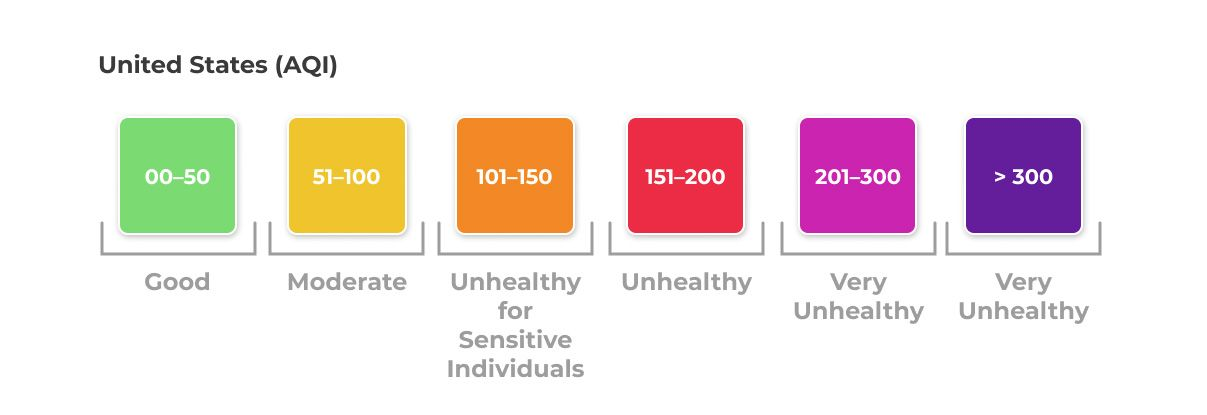
\includegraphics[width=0.9\textwidth]{AQIUSA.jpeg}
    \caption{United States of America Air Quality Standards (EPA, 2025).}
    \label{fig:aqi_usa}
\end{figure}

\subsection{How AQI is Calculated}
\label{sec:calc}

For each pollutant $p$ the concentration $C_p$, averaged over the period prescribed for that pollutant (24 hours for particles, 8 hours for ozone and carbon monoxide, 1 hour for NO$_2$ and SO$_2$) and truncated to the reporting precision, is located between two breakpoints $BP_{Lo} \le C_p \le BP_{Hi}$ and mapped linearly onto the index range $[I_{Lo}, I_{Hi}]$ of the corresponding category \citep{epa2024tad}:
\begin{equation}
I_p = \frac{I_{Hi} - I_{Lo}}{BP_{Hi} - BP_{Lo}}\,\left(C_p - BP_{Lo}\right) + I_{Lo},
\qquad
\text{AQI} = \max_p I_p .
\end{equation}
The overall AQI is therefore the sub-index of the \emph{dominant} pollutant. Table~\ref{tab:bp} gives the PM$_{2.5}$ breakpoints before and after the EPA revision of February 2024, which lowered the ceiling of the ``Good'' category from 12.0 to 9.0~$\mu$g/m$^3$.

\begin{table}[H]
\centering\small
\begin{tabular}{lccc}
\toprule
Category & AQI & PM$_{2.5}$ 24 h, 2012 table ($\mu$g/m$^3$) & PM$_{2.5}$ 24 h, 2024 table ($\mu$g/m$^3$)\\
\midrule
Good & 0--50 & 0.0--12.0 & 0.0--9.0\\
Moderate & 51--100 & 12.1--35.4 & 9.1--35.4\\
Unhealthy for Sensitive Groups & 101--150 & 35.5--55.4 & 35.5--55.4\\
Unhealthy & 151--200 & 55.5--150.4 & 55.5--125.4\\
Very Unhealthy & 201--300 & 150.5--250.4 & 125.5--225.4\\
Hazardous & 301--500 & 250.5--500.4 & 225.5--325.4\\
\bottomrule
\end{tabular}
\caption{US EPA PM$_{2.5}$ breakpoints, implemented in \texttt{aqi2.indices} with the ozone (8 h and 1 h), CO, NO$_2$, SO$_2$ and PM$_{10}$ tables.}
\label{tab:bp}
\end{table}

Other conventions follow different logics. The European Air Quality Index (EEA) assigns six bands from ``Good'' to ``Extremely poor'' to each pollutant and reports the worst one; the Citeair Common Air Quality Index (CAQI) interpolates a continuous 0 to 100+ scale on a common grid \citep{elshout2014}; Canada's Air Quality Health Index (AQHI) \emph{adds} the excess risks of NO$_2$, O$_3$ and PM$_{2.5}$ \citep{stieb2008}:
\begin{equation}
\text{AQHI} = \frac{1000}{10.4}\left[\left(e^{0.000871\,\text{NO}_2}-1\right)+\left(e^{0.000537\,\text{O}_3}-1\right)+\left(e^{0.000487\,\text{PM}_{2.5}}-1\right)\right].
\end{equation}
The WHO 2021 guidelines are not an index but health benchmarks: 15~$\mu$g/m$^3$ for 24-hour PM$_{2.5}$, 5~$\mu$g/m$^3$ for its annual mean \citep{who2021}. All of them are implemented in the \texttt{aqi2} package of this project, with an exact inverse of the EPA breakpoints.

\paragraph{Validation of the engine.} Since 2019 the AirNow files publish the official AQI next to each concentration. Recomputing it for the whole tri-state region reproduces \textbf{\ValOzN{} ozone values exactly}, and PM$_{2.5}$ within one point in \ValPMwithin{}\% of cases (the residual one-point differences come from the rounding of the published concentrations). The comparison also dates the switch to the new PM$_{2.5}$ breakpoints in the AirNow feed: early May 2024.

\subsection{Global vs Local AQI}

A city has no single air quality. Around New York, the variogram of daily concentrations (the mean squared difference between two monitors as a function of their distance) shows that, once the regional level of the day is removed, about half of the remaining PM$_{2.5}$ contrast between monitors is local (near roads, industrial sources), while ozone contrasts vary smoothly over hundreds of kilometres. The EPA reports the AQI of an area as the highest value among its monitors; this study uses instead a \emph{network composite} (the anomaly-method mean of all monitors, robust to monitors joining or leaving) to describe the typical exposure of the city, and continuous maps (Section~\ref{sec:geo}) to describe its geography.

% ===========================================================================
\section{Data Collection and Methodology}
% ===========================================================================

\subsection{Data Sources}

\begin{table}[H]
\centering\small
\begin{tabularx}{\textwidth}{>{\raggedright\arraybackslash}p{4.3cm}>{\raggedright\arraybackslash}Xl}
\toprule
Source & Content & Period\\
\midrule
aqicn.org export (\texttt{NYpollutants.csv}, v1) \citep{aqicn} & daily PM$_{2.5}$, O$_3$, NO$_2$, CO sub-indices for New York & 2014--2025\\
US EPA AirNow files \citep{airnowfiles} & daily 24 h PM$_{2.5}$ and maximum 8 h O$_3$ at every monitor of the tri-state region; hourly files for the June 2023 smoke and a 2024 sample & 2014--Oct 2026\\
NOAA GHCN-Daily and Global Hourly \citep{ghcnd} & temperature, wind, humidity, pressure, precipitation, smoke or haze flags at 7 stations & 2014--Oct 2026\\
UCI Air Quality \citep{devito2008} & hourly reference analyzers (CO, NO$_2$, NO$_x$, benzene) and 5 metal-oxide sensors, Italian city & Mar 2004--Apr 2005\\
Natural Earth 1:10m & coastline, land, lakes, states, counties, NYC boroughs & static\\
\bottomrule
\end{tabularx}
\caption{Data used in version 2. Every dataset is downloaded by the scripts of \texttt{v2/scripts} and a snapshot is stored in \texttt{v2/data}.}
\end{table}

\subsection{Preprocessing and Cleaning}

Version 1 took its two datasets at face value. Version 2 checks each against an independent source; this is where the most consequential findings of the study come from.

\paragraph{The aqicn export holds AQI values, not concentrations.} CO ranges from 1 to 10 and ozone reaches exactly 500, the ceiling of the AQI scale. Version 1 applied concentration breakpoints to these sub-indices; on the days it used, its reading classified \VoneGood{}\% of days as ``Good'' instead of \VtwoGood{}\% (Figure~\ref{fig:qc}).

\paragraph{Three silent failures in the export.} (i) Cross-correlating each column with an independent reference at lags of $-2$ to $+2$ days (the AirNow composite for PM$_{2.5}$ and ozone, the observed wind speed for NO$_2$ and CO) shows that the gaseous pollutants are stamped \emph{one day early}; they are shifted back. (ii) In 2019 ozone sits at the AQI ceiling for months, including in winter, while the monitors never exceeded 99~ppb (AQI 167) in 13 years: \FlagOz{} days are flagged. (iii) From July 2021 to January 2022 the ratio between the export and the network jumps from a stable \StableRatio{} to 5 to 7: a sensor drift, flagged by a robust rolling detector (\FlagPM{} days), which v1 read as the most polluted year of the decade. After quality control the correlation between the export and the network rises from \CorrBefore{} to \CorrAfter.

\paragraph{The regulatory feed needs checks too.} An automatic filter removes physically impossible values and stuck instruments (five or more identical consecutive days): the Pfizer Lab ozone monitor in the Bronx reported 0~ppb throughout 2014, which would otherwise have faked a strong upward ozone trend. The feed also has reporting gaps (no NYC monitor from February to May 2019); they are bridged by a two-stage model of the regional network (linear fit on the composite of the monitors within 80~km plus gradient-boosted corrections), validated by holding out whole months (R$^2$ \FillRtwoPM{} for PM$_{2.5}$, \FillRtwoOz{} for ozone).

\paragraph{The UCI file.} Version 1 parsed the decimal commas incorrectly, so the missing-value code $-200$ survived in five columns (18\% of the CO ``measurements''), and filled every other gap with a single number, 457.1. Its random forest scored MAE \VoneRFmae{} on CO mostly by learning these codes. The benzene ``reference'' turns out to be a fourth-degree polynomial of one cheap sensor (R$^2$ = \BenzeneRtwo): it was estimated, not measured, and is excluded from the benchmarks.

\begin{figure}[H]
\centering
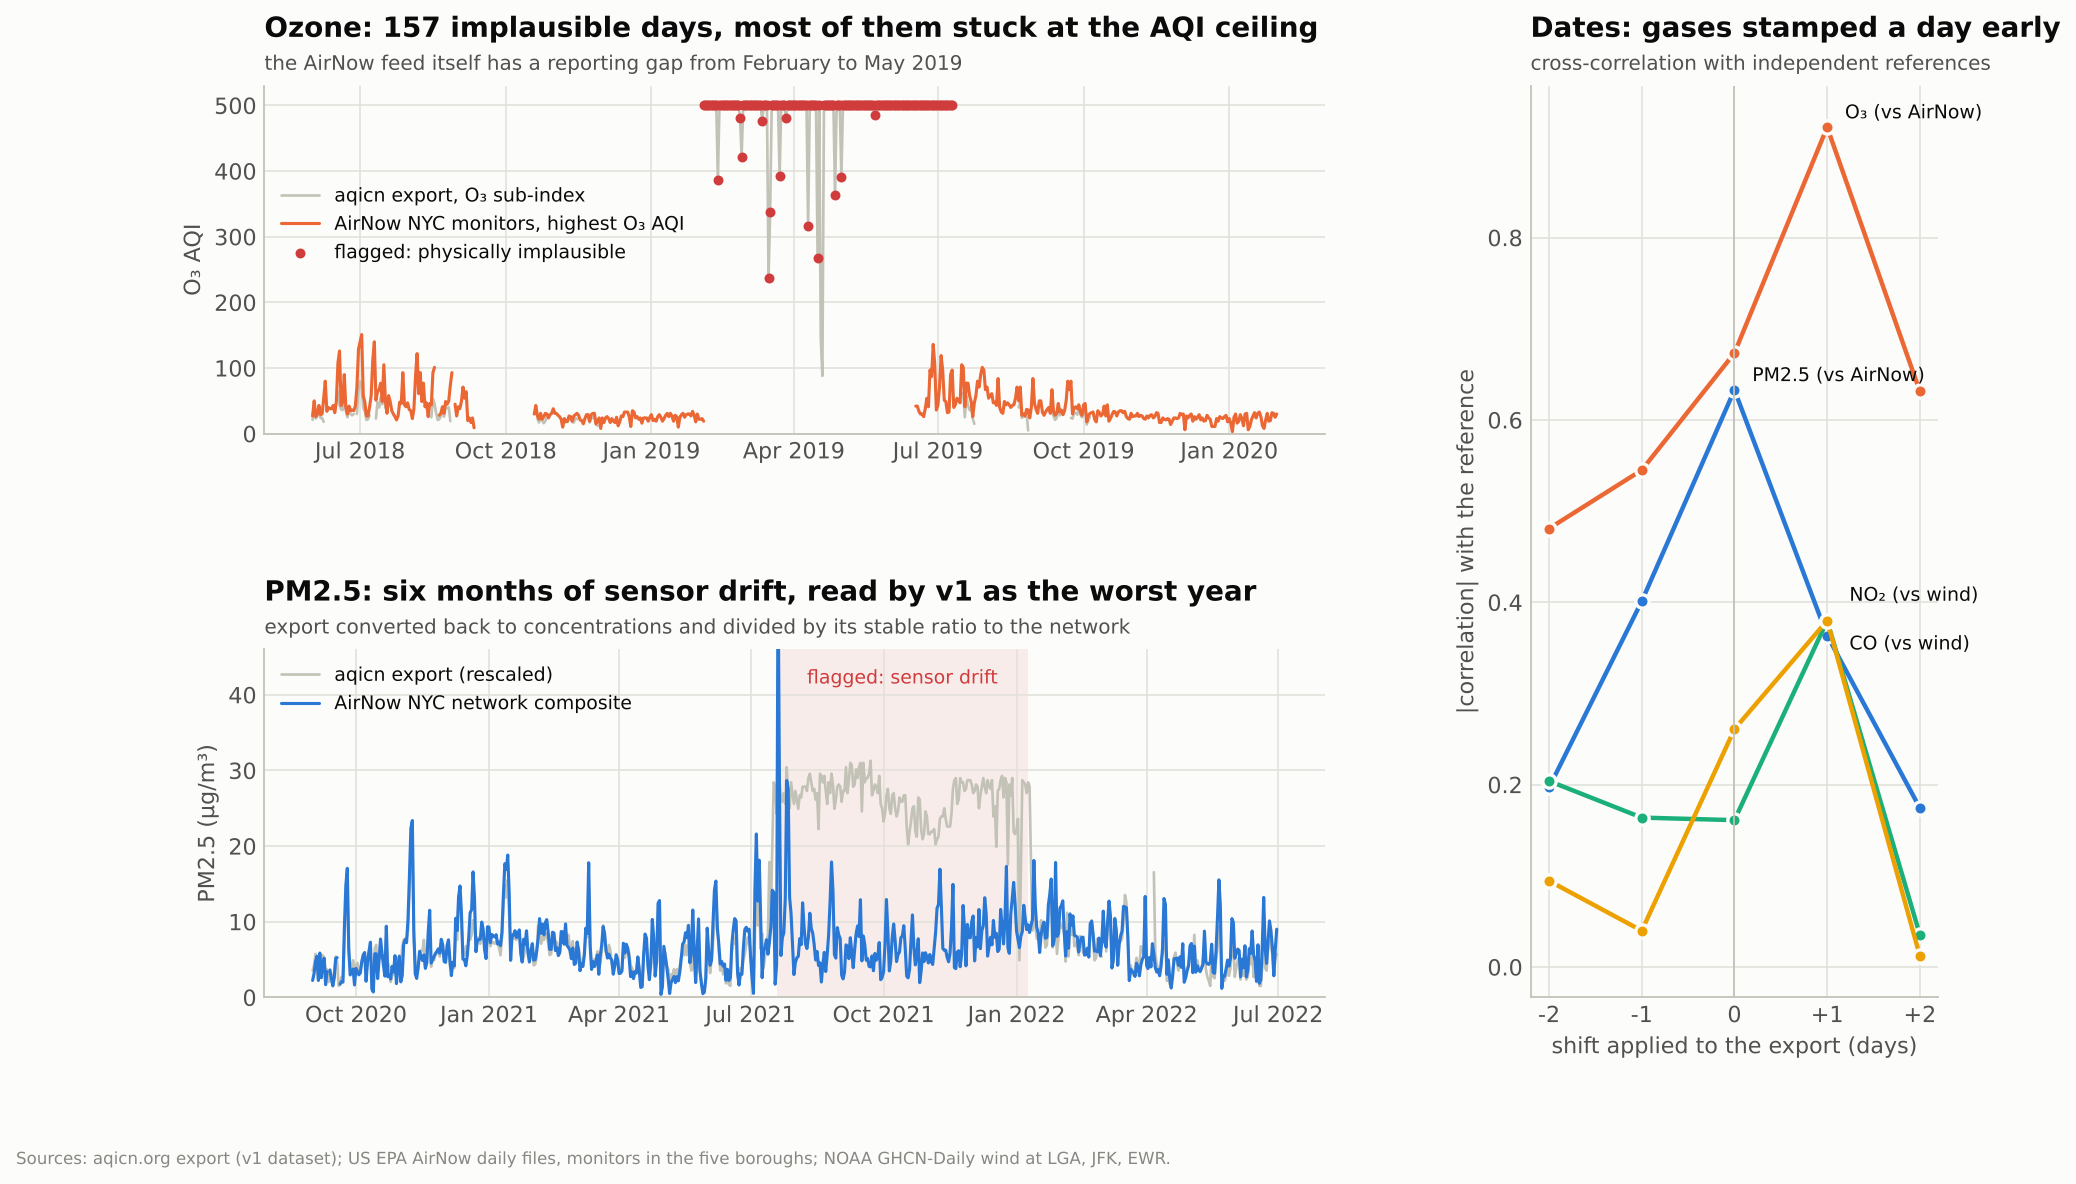
\includegraphics[width=\textwidth]{01_quality_control.png}
\caption{Quality control of the aqicn export against independent references.}
\label{fig:qc}
\end{figure}

\subsection{Feature Selection}

Forecasting features describe the state of the air at issue time (lags of 0 to 6 days or 0 to 24 hours, rolling means, maxima and standard deviations, exponential averages), the other pollutants, the weather (temperature, wind components, gusts, precipitation, humidity, pressure), the calendar of the target time (cyclical day of year and hour, weekday, holidays, fireworks days) and, in the spatial models, geography (coordinates, distance to Midtown and to the coast). Rather than pruning features a priori, the gradient-boosting models are regularised and explained after the fact with exact TreeSHAP contributions \citep{lundberg2020}: yesterday's level dominates PM$_{2.5}$, tomorrow's maximum temperature dominates ozone, and humidity and temperature dominate the corrections of the low-cost sensors.

\subsection{Machine Learning Models Used}

\begin{itemize}
\item \textbf{Gradient boosting} (LightGBM, \citealp{ke2017}) with quantile losses (10\%, 50\%, 90\%) for probabilistic forecasting, calibrated by \textbf{conformalised quantile regression} \citep{romano2019} on the most recent 20\% of the training period, so that the 80\% intervals cover 80\% of outcomes.
\item \textbf{Meteorological normalisation} \citep{grange2019}: a boosting model learns pollution from weather, season and time; predictions are averaged over 300 resampled weather and calendar conditions to leave only the time trend, summarised with the Theil-Sen slope and the Mann-Kendall test \citep{sen1968} on STL-deseasonalised monthly means \citep{cleveland1990}.
\item \textbf{Counterfactual analysis} of the COVID-19 lockdown with an \textbf{in-time placebo test}: the same model is evaluated on the same spring window of every other year to measure the noise floor of the method.
\item \textbf{Virtual sensing}: calibration of the UCI metal-oxide sensors against the reference analyzers with ridge regression and LightGBM, under four recalibration schedules.
\item \textbf{Spatial prediction}: inverse distance weighting, ordinary kriging with a pooled variogram, Gaussian processes with daily maximum-likelihood hyperparameters \citep{rasmussen2006}, Random Forest Spatial Interpolation (RFSI, \citealp{sekulic2020}) with LightGBM, and a hybrid where boosting learns the kriging leave-one-out residuals \citep{dubrule1983}.
\end{itemize}
All evaluations respect time and space: walk-forward (expanding window) for forecasts, grouped cross-validation by monitor for maps.

% ===========================================================================
\section{Results}
% ===========================================================================

\subsection{Model Performance}

\paragraph{Forecasting the New York AQI.} Each test year from 2021 to 2026 is predicted by a model trained only on earlier years. Table~\ref{tab:fc} reports the day-ahead scores; the skill score is $1 - \text{MAE}/\text{MAE}_{\text{baseline}}$.

\begin{table}[H]
\centering\small
\begin{tabular}{llcccc}
\toprule
Target & Setting & MAE & Skill vs persistence & Skill vs climatology & 80\% coverage\\
\midrule
PM$_{2.5}$ ($\mu$g/m$^3$) & operational & \FcPMopMAE & \FcPMopSkP\% & \FcPMopSkC\% & \FcPMopCov\%\\
PM$_{2.5}$ ($\mu$g/m$^3$) & with weather forecast & \FcPMwxMAE & \FcPMwxSkP\% & \FcPMwxSkC\% & \FcPMwxCov\%\\
Ozone (ppb) & operational & \FcOzopMAE & \FcOzopSkP\% & \FcOzopSkC\% & \FcOzopCov\%\\
Ozone (ppb) & with weather forecast & \FcOzwxMAE & \FcOzwxSkP\% & \FcOzwxSkC\% & \FcOzwxCov\%\\
\bottomrule
\end{tabular}
\caption{Day-ahead forecasts of the New York network composites, walk-forward 2021--2026. Raw quantile intervals covered only about \RawCov\% of outcomes; conformal calibration restores the nominal level.}
\label{tab:fc}
\end{table}

The AQI category of the next day is right \CatAcc\% of the time (persistence: \CatAccPers\%). Days above AQI 100 remain hard: they are mostly smoke onsets, which local data cannot anticipate. Trained on all data up to the last complete day, the operational model issued a live forecast of AQI \LiveAQI{} (\LiveCat) for \LiveDate.

\begin{figure}[H]
\centering
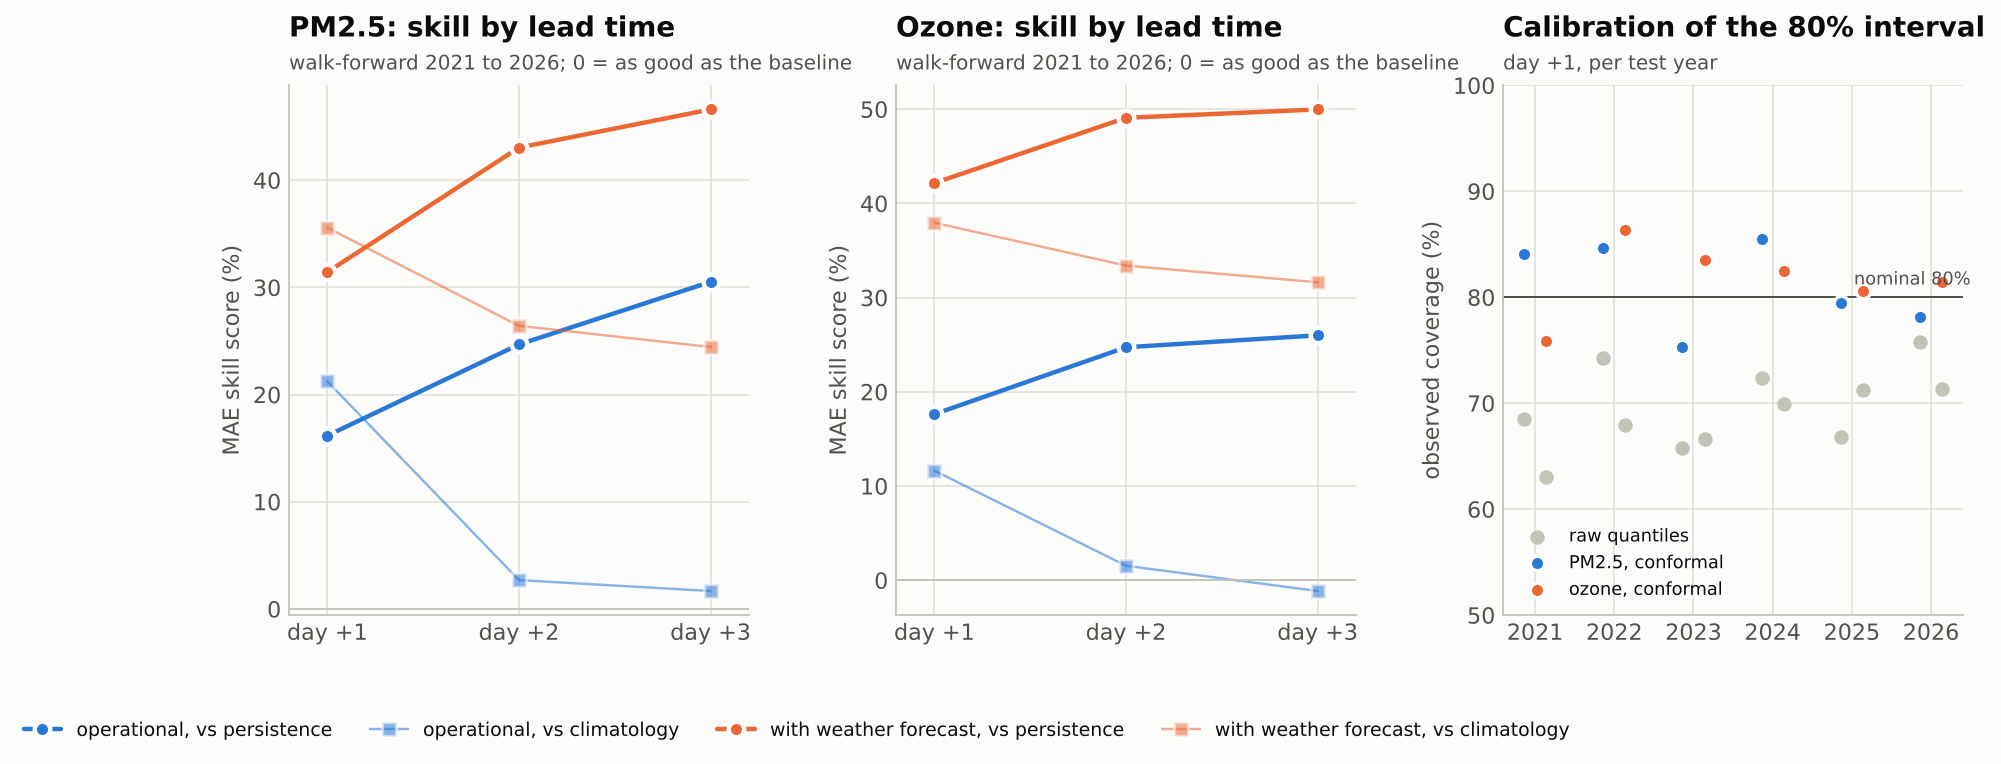
\includegraphics[width=\textwidth]{01_forecast_skill.png}
\caption{Forecast skill by lead time and calibration of the conformal intervals.}
\end{figure}

\paragraph{Low-cost sensors (UCI).} A calibration made once on the first month loses most of its skill for NO$_2$ and NO$_x$ within a few months, while monthly recalibration keeps it (Table~\ref{tab:vs}); the CO sensor is the exception. With monthly recalibration, the CAQI computed from the cheap sensors matches the reference level \LowCostExact\% of the hours and is within one level \LowCostOne\% of the time. Used to fill gaps of the reference analyzers, the virtual sensors halve the error of interpolation and climatology. The hourly CAQI forecast beats persistence at every lead time from 1 to 24 hours.

\begin{table}[H]
\centering\small
\begin{tabular}{llcccc}
\toprule
Target & Model & static & quarterly & monthly & weekly\\
\midrule
CO & LightGBM & 0.88 & 0.75 & 0.83 & 0.86\\
CO & linear & $-$0.25 & 0.57 & 0.77 & 0.83\\
NO$_2$ & LightGBM & 0.34 & 0.66 & 0.72 & 0.79\\
NO$_2$ & linear & 0.24 & 0.25 & 0.66 & 0.80\\
NO$_x$ & LightGBM & 0.07 & 0.80 & 0.87 & 0.90\\
NO$_x$ & linear & $-$0.50 & 0.73 & 0.79 & 0.89\\
\bottomrule
\end{tabular}

\caption{Out-of-sample R$^2$ of the virtual sensors over the 11 months following the first co-location month.}
\label{tab:vs}
\end{table}

\paragraph{Spatial prediction.} Under an 8-fold spatial cross-validation (each group of monitors predicted from the others, on 300 random days and the five worst days), the Gaussian process is the best PM$_{2.5}$ interpolator (RMSE \GeoPMgp~$\mu$g/m$^3$, R$^2$ \GeoPMgpR) and kriging corrected by a boosted residual model is the best for ozone (RMSE \GeoOzbest~ppb, R$^2$ \GeoOzbestR). A purely learned interpolator (RFSI) does not beat geostatistics: with tens of monitors and a smooth regional field, the information lies in the neighbours.

\begin{figure}[H]
\centering
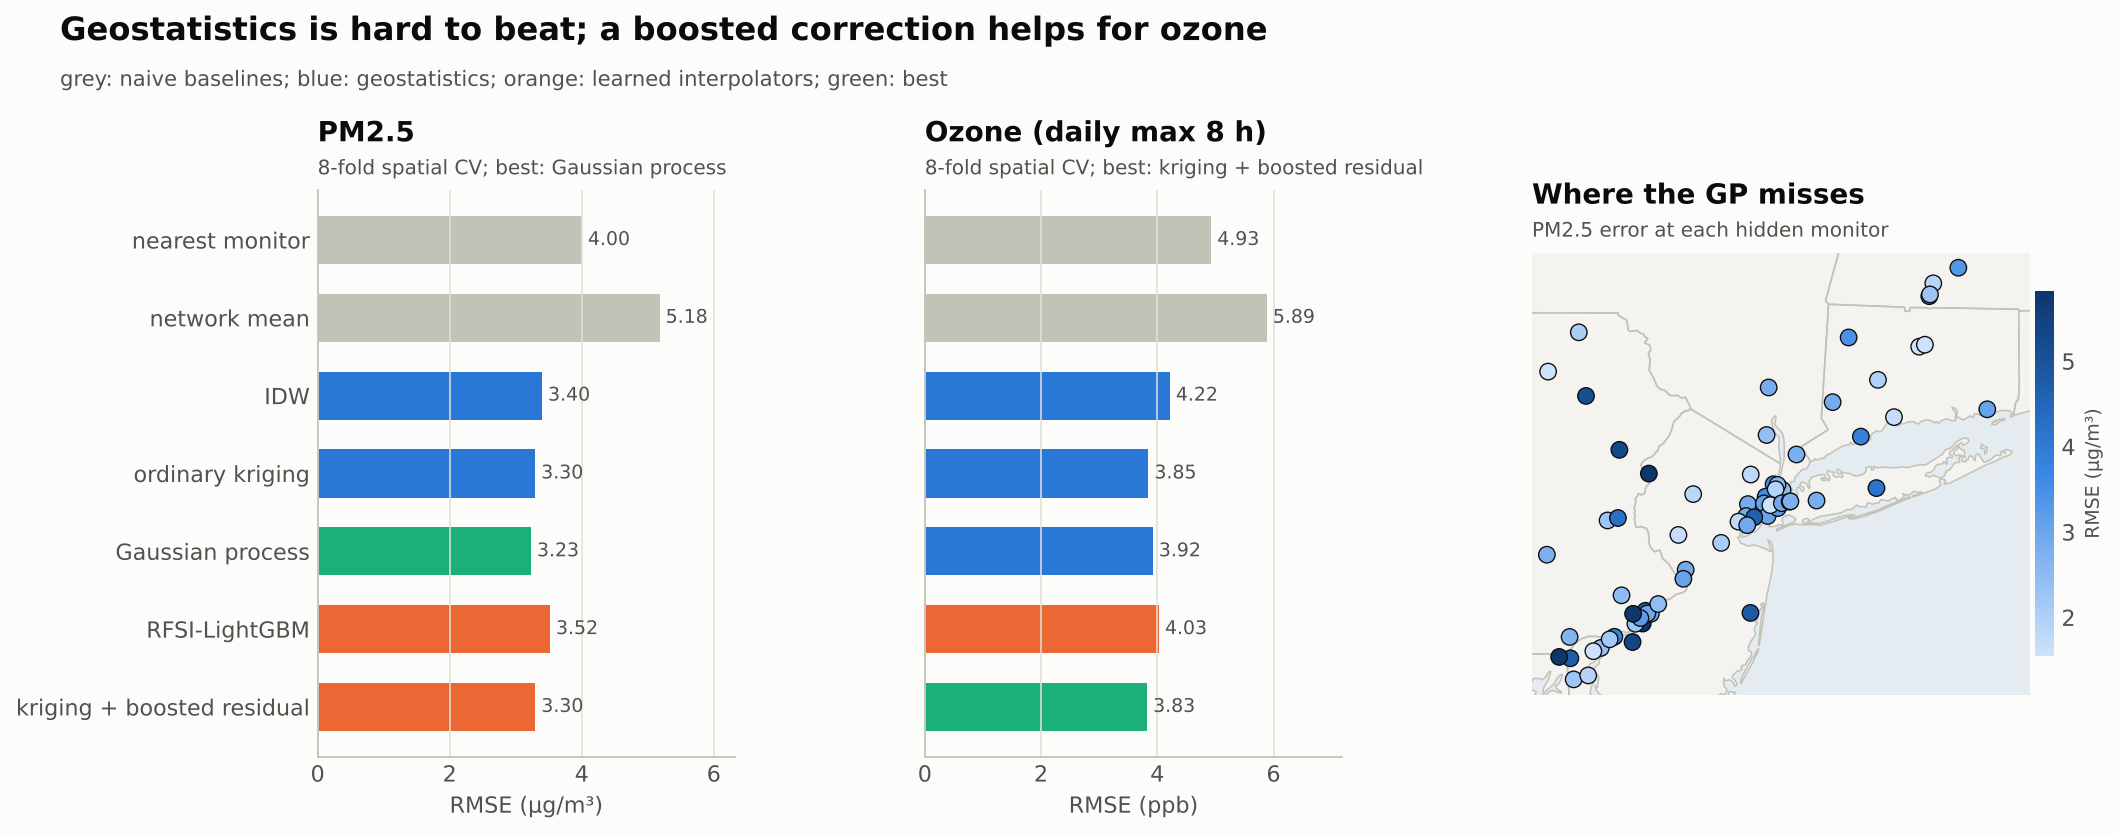
\includegraphics[width=\textwidth]{03_benchmark.png}
\caption{Spatial cross-validation of seven interpolators.}
\end{figure}

\subsection{Comparison with Existing AQI Predictions}

Two references anchor the results. First, the official values: the engine reproduces the AQI published by AirNow (exactly for ozone). Second, the operational baselines that any forecast must beat: persistence, which public forecasts implicitly compete with, and climatology. The gradient-boosting forecasts beat both at every lead time; their main added value comes from weather forecasts for ozone (skill rising from \FcOzopSkP\% to \FcOzwxSkP\% against persistence), much less for particles, whose episodes are driven by transported smoke.

\subsection{Case Studies on Specific Regions}
\label{sec:standards}

\paragraph{Same air, different verdicts.} Over 2014--2026, New York's air is ``Good'' on \ShareGoodTwelve\% of days under the 2012 EPA table, \ShareGoodTwentyFour\% under the 2024 table and only \ShareGoodEEA\% under the European index; the WHO 24-hour PM$_{2.5}$ guideline is exceeded between \WhoMin{} and \WhoMax{} days per year (Figure~\ref{fig:standards}).

\begin{figure}[H]
\centering
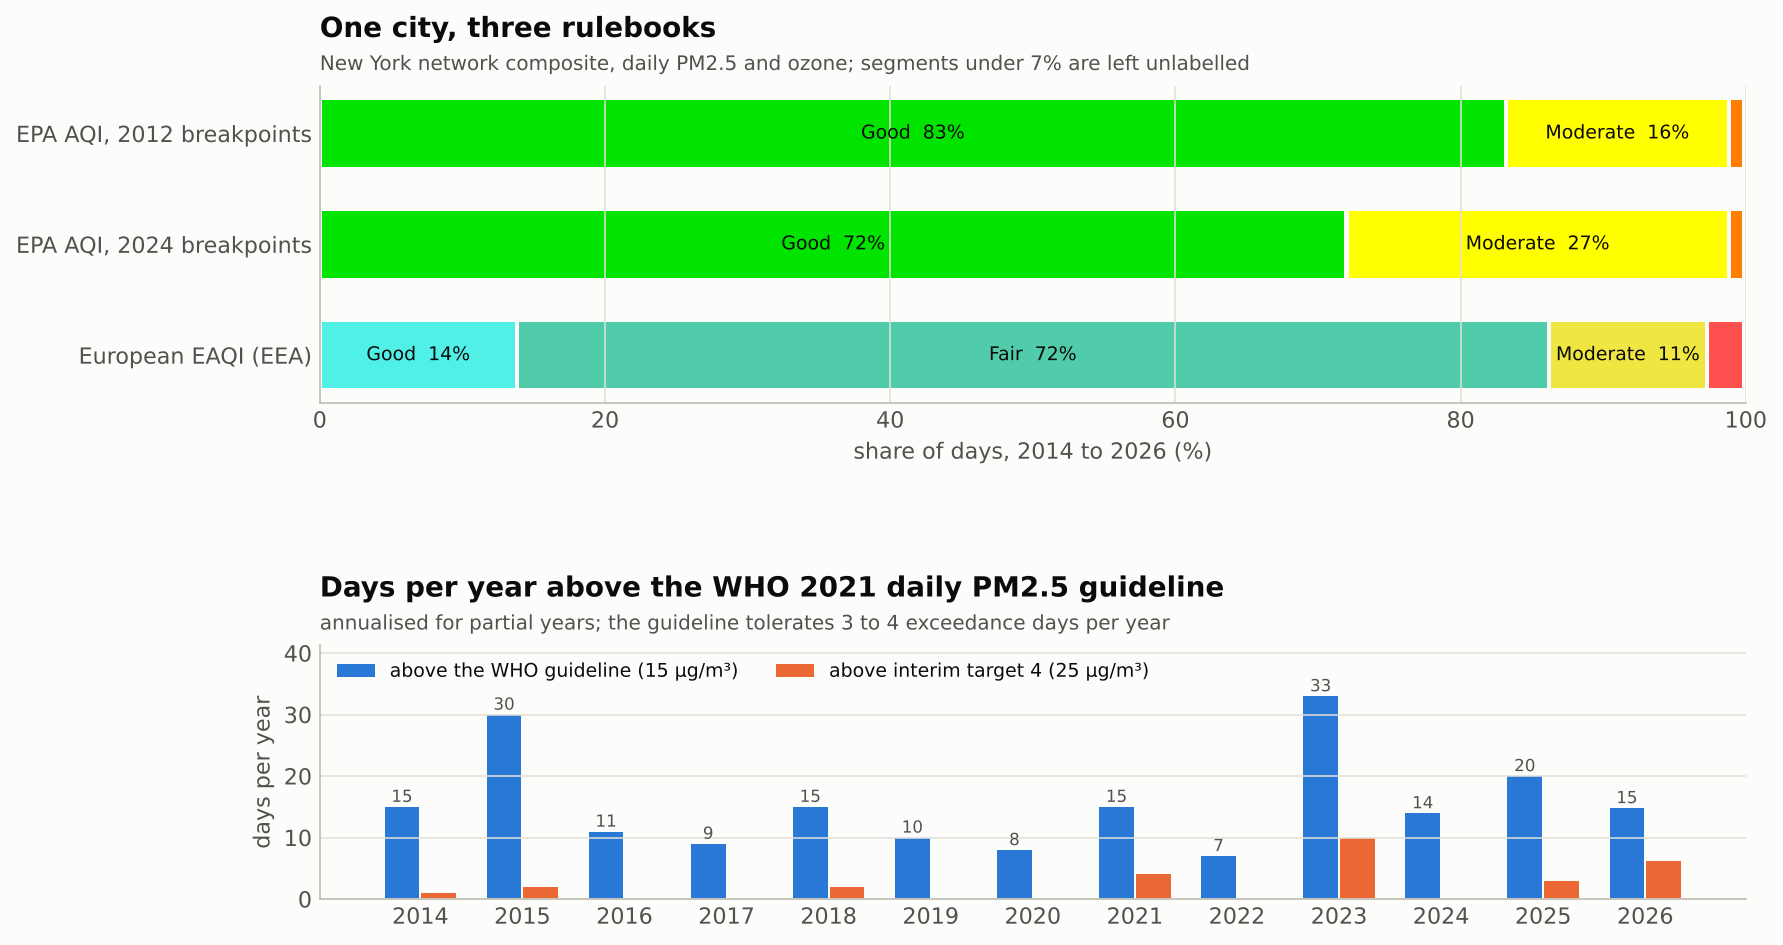
\includegraphics[width=\textwidth]{01_standards_comparison.png}
\caption{The same 13 years judged by three indices and by the WHO guideline.}
\label{fig:standards}
\end{figure}

\paragraph{Trends.} Once the weather is removed, PM$_{2.5}$ shows no significant trend since 2014 (\TrendPM~$\mu$g/m$^3$ per year) while ozone rises by \TrendOz~ppb per year (\TrendOzPct\% per year, Mann-Kendall $p$ \TrendOzP). Rising urban ozone alongside falling NO$_x$ emissions is the signature of reduced titration, also visible in space (Section~\ref{sec:geo}).

\paragraph{Episodes.} The worst day of the record is June 7, 2023, when Quebec wildfire smoke drove the city-wide 24-hour PM$_{2.5}$ to \WorstPM~$\mu$g/m$^3$ (AQI \WorstAQI, ``Very Unhealthy''); a second regionally coherent haze episode reached AQI \SecondAQI{} in mid-July 2026. Independence Day fireworks add a median \FireworksPM~$\mu$g/m$^3$ to the city-wide daily mean, New Year's fireworks leave no detectable mark. During the spring 2020 lockdown, NO$_2$ was \CovidNOtwo\% below its business-as-usual counterfactual, outside the range of every placebo year (\PlaceboNOmin\% to \PlaceboNOmax\%); PM$_{2.5}$ was \CovidPM\% below, also beyond its placebo range (\PlaceboPMmin\% to \PlaceboPMmax\%), an estimate that includes the regional drop of upwind emissions and is less precise.

\begin{figure}[H]
\centering
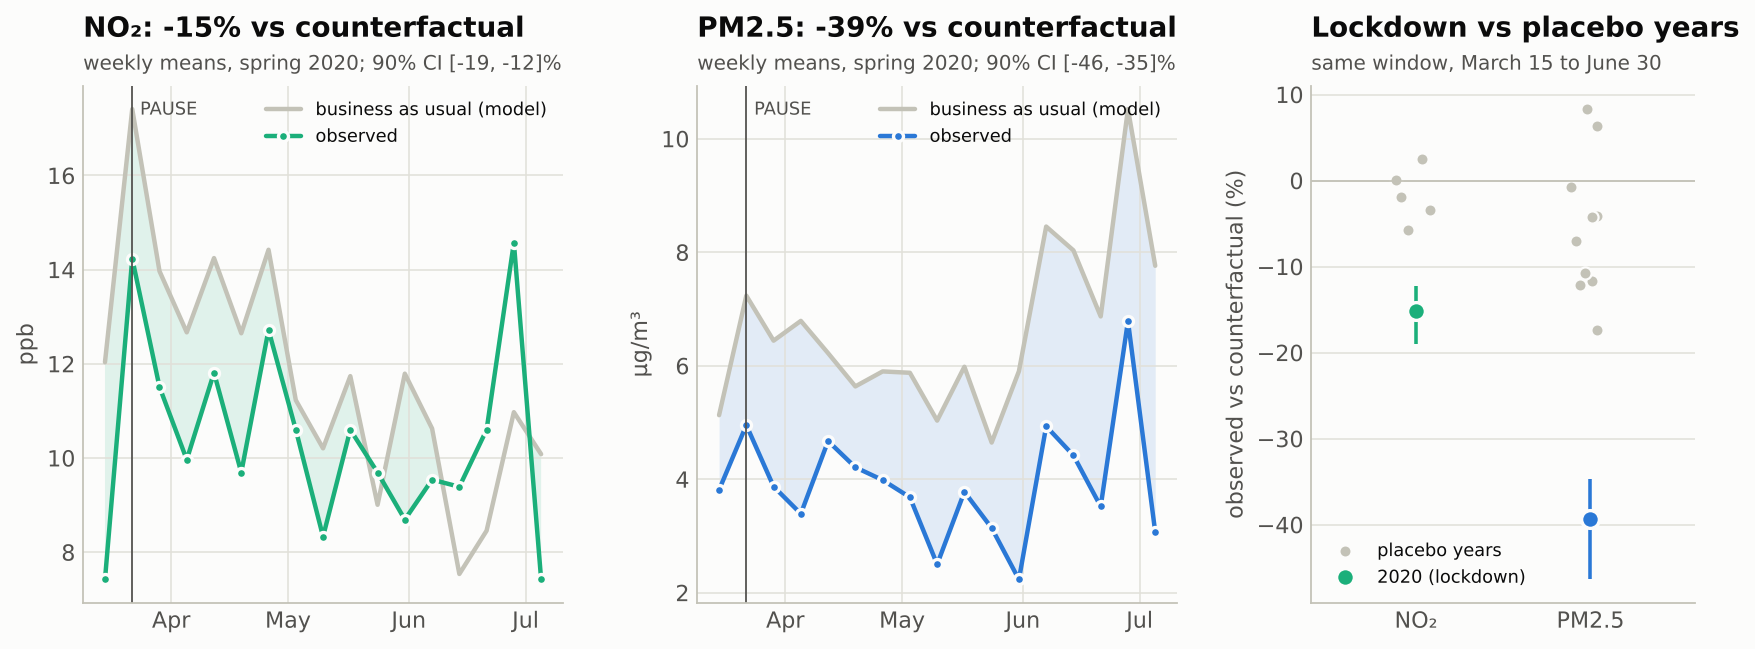
\includegraphics[width=\textwidth]{01_covid_counterfactual.png}
\caption{The COVID-19 lockdown against a business-as-usual counterfactual and against placebo years.}
\end{figure}

\paragraph{Geospatial prediction.}
\label{sec:geo}
Continuous maps reveal the two faces of urban air (Figure~\ref{fig:maps}): fine particles follow the urban corridor from Philadelphia to New York, ozone peaks downwind of the city along the Connecticut shore because fresh NO emissions destroy it in the core. Summing the daily Gaussian-process probabilities of exceeding a threshold gives the expected number of exceedance days at every location, monitored or not. Weighted by the 2020 Census, New Yorkers breathed a population-weighted PM$_{2.5}$ of \PopPM~$\mu$g/m$^3$ in 2025, \PopRatio{} times the WHO annual guideline.

\begin{figure}[H]
\centering
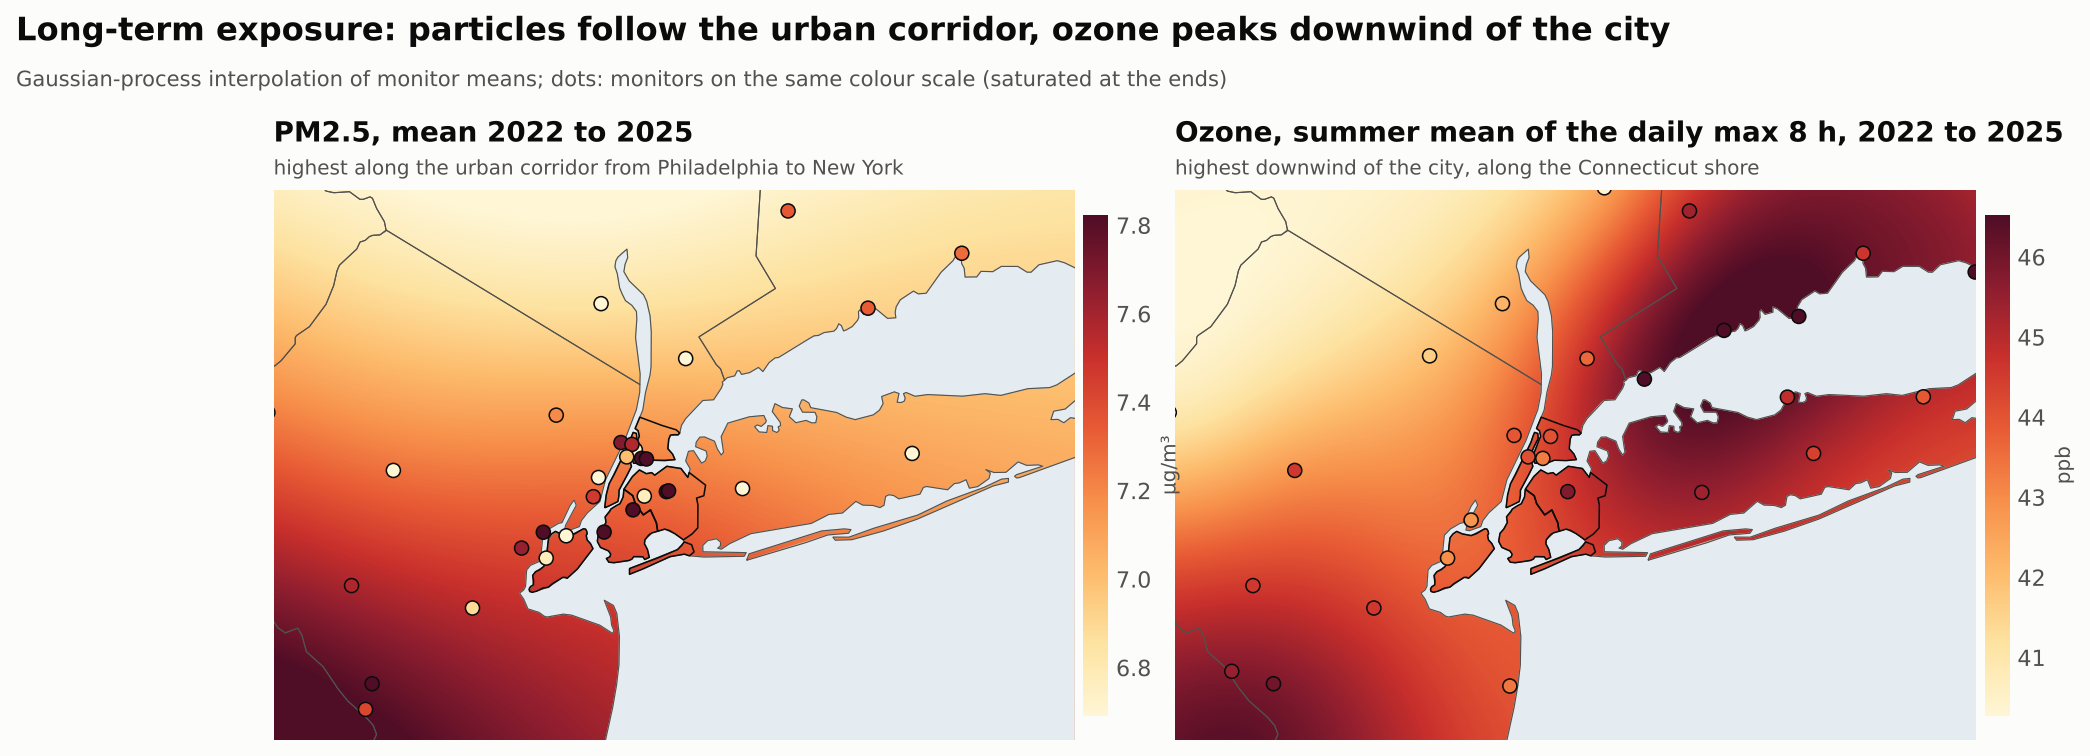
\includegraphics[width=\textwidth]{03_longterm_maps.png}
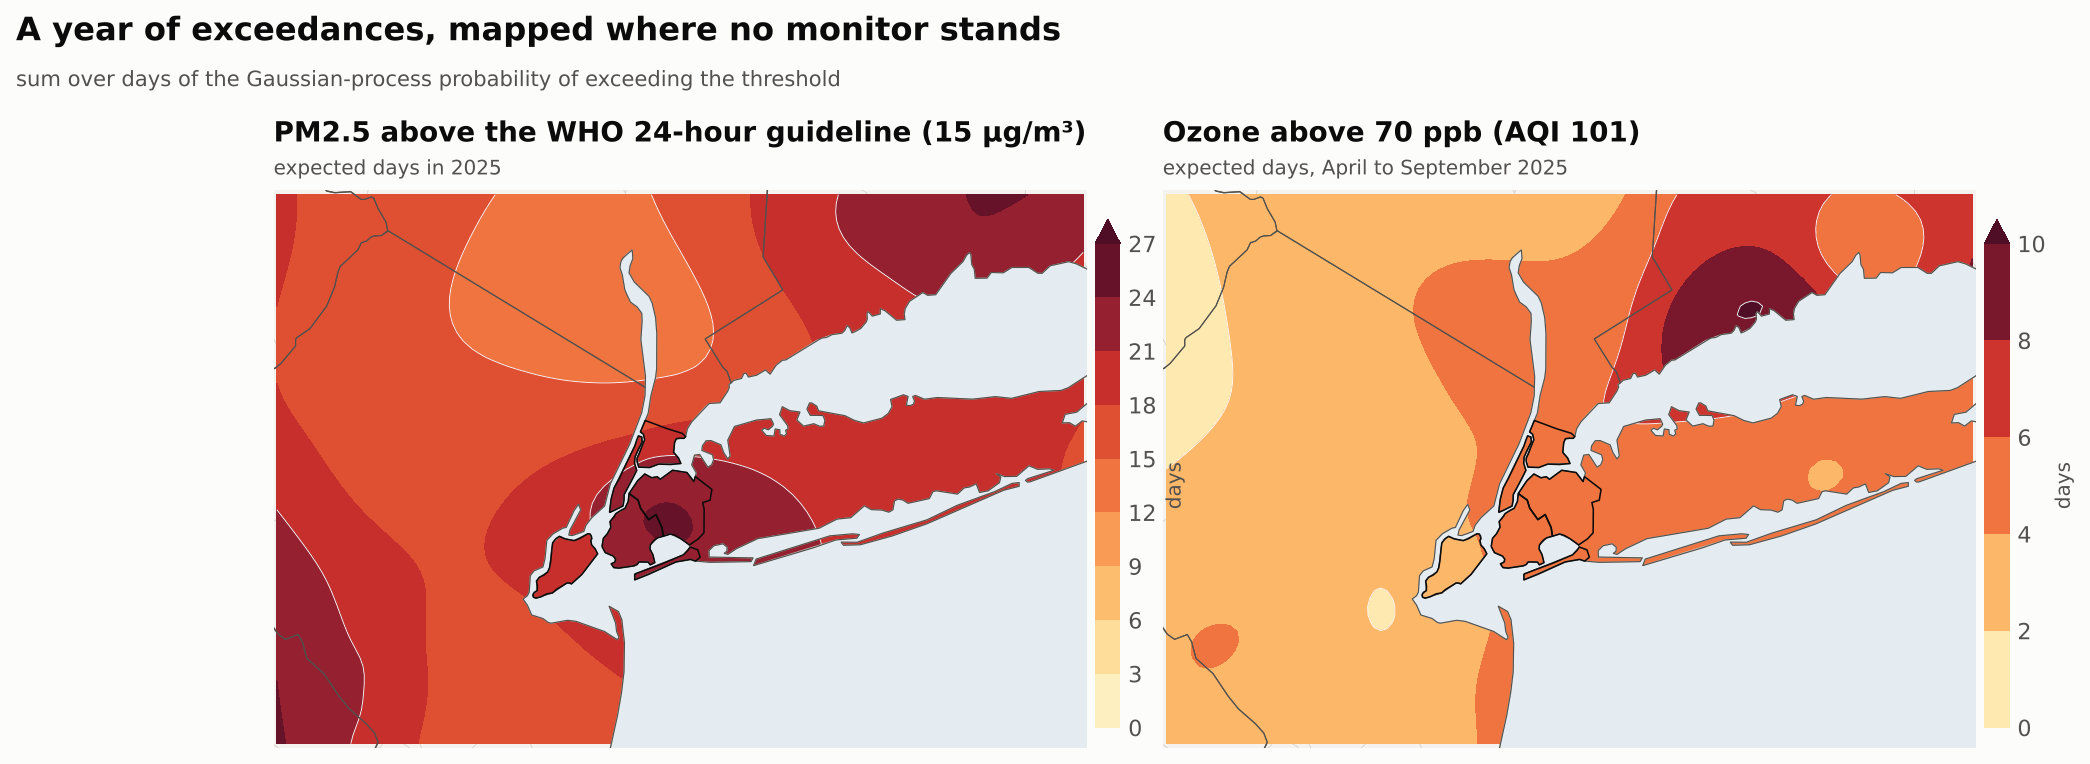
\includegraphics[width=\textwidth]{03_exceedance_maps.png}
\caption{Long-term exposure (top) and expected exceedance days in 2025 (bottom).}
\label{fig:maps}
\end{figure}

\begin{figure}[H]
\centering
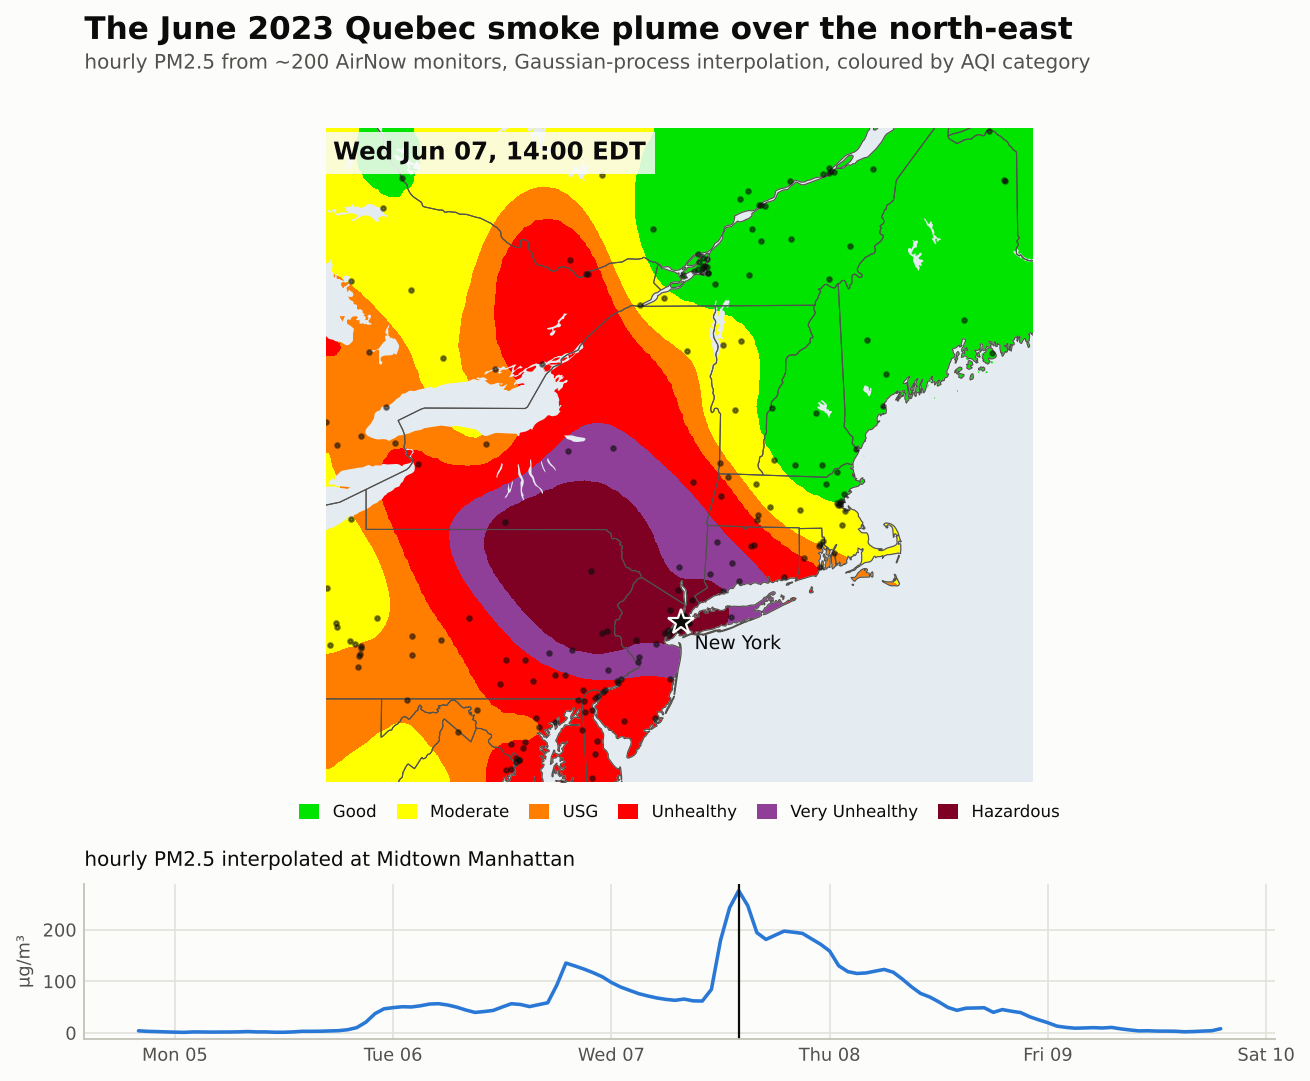
\includegraphics[width=0.75\textwidth]{03_smoke_peak_frame.png}
\caption{The June 2023 smoke plume at its peak over New York (one frame of the hourly animation \texttt{figures/03\_smoke\_june2023.gif}).}
\end{figure}

% ===========================================================================
\section{Discussion}
% ===========================================================================

\subsection{Interpretation of Results}

The most important results of this version are not model scores but data findings: the v1 dataset was read on the wrong scale, carried a one-day shift on its gases and two long sensor failures, and even the regulatory feed contained a monitor stuck at zero. Each of them changes a conclusion (``2021 was the worst year'', ``ozone is rising fast''). Cross-checking against independent sources is therefore the first modelling step, not a preliminary.

On modelling, the results favour simple structure with honest validation: gradient boosting beats persistence and climatology, conformal calibration is needed to make its intervals trustworthy, and for spatial prediction the Gaussian process is hard to beat, learning paying off only as a correction of kriging. Weather is the dominant short-term driver of ozone, while particle episodes are driven by transported smoke.

\subsection{Limitations of the Study}

\begin{itemize}
\item AirNow data are real-time and preliminary; the final regulatory archive (EPA AQS) may differ slightly.
\item The weather used as ``forecast'' is the observed weather of the target day, an upper bound on the value of a real weather forecast.
\item With about 60 monitors, the maps cannot resolve street-level gradients of PM$_{2.5}$, and NO$_2$ is not measured inside New York City in the AirNow feed.
\item The UCI dataset covers one year, one city and one sensor box; drift rates may differ for newer sensors.
\item Population weighting uses borough totals, not a population grid.
\end{itemize}

\subsection{Potential Improvements}

Smoke transport forecasts (for instance from operational smoke models) and satellite aerosol optical depth would address the main weakness of the forecasts, the onset of smoke episodes. Land-use covariates (traffic, building density) and the NYC Community Air Survey would give the spatial models information that the monitors do not share. A population grid would refine the exposure estimates.

% ===========================================================================
\section{Conclusion and Potential Improvements}
% ===========================================================================

\subsection{Summary of Findings}

\begin{itemize}
\item Version 1's New York data were AQI sub-indices, not concentrations; three silent failures (a one-day shift, an ozone plateau, a PM$_{2.5}$ drift) are detected and corrected against EPA and NOAA data.
\item A multi-standard AQI engine reproduces the official AirNow values and shows how much the verdict depends on the rulebook.
\item Since 2014, weather-normalised PM$_{2.5}$ is flat while ozone rises; the COVID-19 lockdown cut NO$_2$ by \CovidNOtwo\% against its counterfactual.
\item Probabilistic forecasts beat persistence and climatology with calibrated intervals; a live forecast is produced from the latest data.
\item Low-cost sensors become reliable virtual analyzers only with regular recalibration.
\item Continuous maps quantify exposure and exceedance probabilities where no monitor stands.
\end{itemize}

\subsection{Applications in Policy and Urban Planning}

Exceedance-probability maps indicate where new monitors would reduce uncertainty most and where sensitive facilities (schools, hospitals) face the most exceedance days. Weather-normalised trends and counterfactuals evaluate policies (traffic restrictions, congestion pricing) without being fooled by a mild or a hot year. The comparison of indices shows that switching from the EPA scale to WHO-aligned thresholds would change the public message on a large share of days, a choice that is political as much as scientific.

\subsection{Next Steps in Research}

Integrating smoke forecasts and satellite data into the forecasting model; extending the spatial model with land-use covariates and dense low-cost networks, calibrated with the drift-aware schedule found here; and estimating health impacts from the exposure maps with concentration-response functions.

\bibliographystyle{plainnat}
\bibliography{references}

\end{document}
